\documentclass[8pt,a4paper,compress,handout]{beamer}

\usepackage{/home/siyer/lib/slides}

\title{Modules and Clients}
\date{}

\begin{document}
\begin{frame}
\vfill
\titlepage
\end{frame}

\begin{frame}
\frametitle{Outline}
\tableofcontents
\end{frame}

\section{.}
\begin{frame}[fragile]
\begin{framed}
\tiny gaussian.py: Accept floats $z$, $mu$, and $sigma$ as command-line arguments. Use them to test the \lstinline{phi()} and \lstinline{Phi()} functions. Write the results to standard output.
\end{framed}

\begin{lstlisting}[language=Python]
import math
import stdio
import sys

def pdf(x, mu = 0.0, sigma = 1.0):
    x = float(x - mu) / sigma
    return math.exp(- x * x / 2.0) / math.sqrt(2.0 * math.pi) / sigma

def cdf(z, mu = 0.0, sigma = 1.0):
    z = float(z - mu) / sigma
    if z < -8.0: return 0.0
    if z > +8.0: return 1.0
    total = 0.0
    term = z
    i = 3
    while total != total + term:
        total += term
        term *= z * z / i
        i += 2
    return 0.5 + total * pdf(z)
\end{lstlisting}
\end{frame}

\begin{frame}[fragile]
\begin{lstlisting}[language=Python]
def main():
    z = float(sys.argv[1])
    mu = float(sys.argv[2])
    sigma = float(sys.argv[3])
    stdio.writeln(cdf(z, mu, sigma))

if __name__ == '__main__':
    main()
\end{lstlisting}

\begin{lstlisting}[language={}]
$ python gaussian.py 820 1019 209
0.170509668691
$ python gaussian.py 1500 1019 209
0.989316483738
$ python gaussian.py 1500 1025 231
0.980122090737
\end{lstlisting}
\end{frame}

\begin{frame}[fragile]
\begin{framed}
\tiny gaussiantable.py:  Accept a mean and standard deviation as command-line arguments. Write to standard output a table of the percentage of students scoring below certain scores on the SAT, assuming the test scores obey a Gaussian  distribution with the given mean and standard deviation.
\end{framed}

\begin{lstlisting}[language=Python]
import gaussian
import stdio
import sys

def main():
    mu = float(sys.argv[1])
    sigma = float(sys.argv[2])
    for score in range(400, 1600 + 1, 100):
        percent = 100 * gaussian.cdf(score, mu, sigma)
        stdio.writef('%4d  %.2f\n', score, percent)
 
if __name__ == '__main__':
    main()
\end{lstlisting}

\begin{lstlisting}[language={}]
$ python gaussiantable.py 1019 209
 400  0.15
 500  0.65
 600  2.25
 700  6.35
 800  14.74
 900  28.45
1000  46.38
1100  65.08
1200  80.68
1300  91.06
1400  96.58
1500  98.93
1600  99.73
\end{lstlisting}
\end{frame}

\begin{frame}[fragile]
\begin{framed}
\tiny sierpinski.py: Accept integer $n$ as a command-line argument. Play the chaos game on a triangle to produce Sierpinski triangle of $n$ points.
\end{framed}

\begin{lstlisting}[language=Python]
import stddraw
import stdrandom
import sys

def main():
    n = int(sys.argv[1])
    cx = [0.000, 1.000, 0.500]
    cy = [0.000, 0.000, 0.866]
    x = 0.0
    y = 0.0
    stddraw.setPenRadius(0.0)
    for i in range(n):
        r = stdrandom.uniformInt(0, 3)
        x = (x + cx[r]) / 2.0
        y = (y + cy[r]) / 2.0
        stddraw.point(x, y)
    stddraw.show()

if __name__ == '__main__':
    main()
\end{lstlisting}

\begin{minipage}{160pt}
\begin{lstlisting}[language={}]
$ python sierpinski.py 20000
\end{lstlisting}
\end{minipage}%
\begin{minipage}{140pt}
\hfill 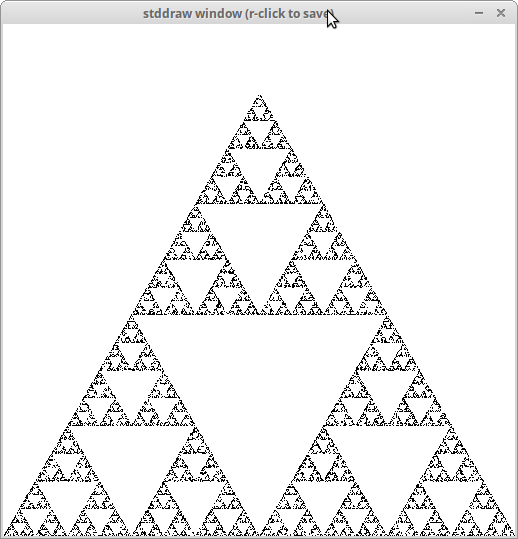
\includegraphics[scale=0.12]{figures/sierpinski.png}
\end{minipage}
\end{frame}

\begin{frame}[fragile]
\begin{framed}
\tiny ifs.py: Accept integer $n$ as a command-line argument. Read a $1$-by-$m$ vector (probabilities) and two $m$-by-$3$ matrices (coefficients for updating $x$ and $y$, respectively) from standard input. Plot the results as a set of $n$ points to standard draw.
\end{framed}

\begin{lstlisting}[language=Python]
import stdarray
import stddraw
import stdrandom
import sys

def main():
    n = int(sys.argv[1])
    dist = stdarray.readFloat1D()
    cx = stdarray.readFloat2D()
    cy = stdarray.readFloat2D()
    x = 0.0
    y = 0.0
    stddraw.setPenRadius(0.0)
    for i in range(n):
        r = stdrandom.discrete(dist)
        x0 = cx[r][0] * x + cx[r][1] * y + cx[r][2]
        y0 = cy[r][0] * x + cy[r][1] * y + cy[r][2]
        x = x0
        y = y0
        stddraw.point(x, y)
    stddraw.show()

if __name__ == '__main__':
    main()
\end{lstlisting}
\end{frame}

\begin{frame}[fragile]
Sierpinski triangle:

\begin{minipage}{160pt}
\begin{lstlisting}[language={}]
$ more sierpinski.txt
3   
  .33 .33 .34 
3 3 
  .50 .00 .00 
  .50 .00 .50 
  .50 .00 .25 
3 3 
  .00 .50 .00 
  .00 .50 .00 
  .00 .50 .433 
$ python ifs.py 20000 < sierpinski.txt
\end{lstlisting}
\end{minipage}%
\begin{minipage}{140pt}
\begin{center}
\hfill 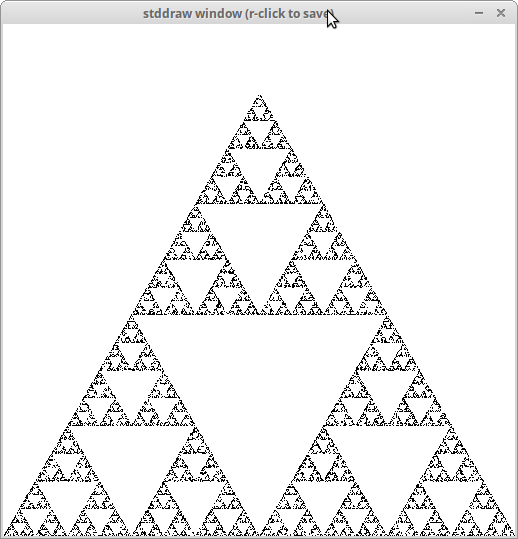
\includegraphics[scale=0.17]{figures/sierpinski.png}
\end{center}
\end{minipage}

\bigskip

Barnsley fern:

\begin{minipage}{160pt}
\begin{lstlisting}[language={}]
$ more barnsley.txt
4
   0.01  0.85  0.07  0.07
4 3
   0.00  0.00  0.500
   0.85  0.04  0.075
   0.20 -0.26  0.400
  -0.15  0.28  0.575
4 3
   0.00  0.16  0.000
  -0.04  0.85  0.180
   0.23  0.22  0.045
   0.26  0.24 -0.086
$ python ifs.py 20000 < barnsley.txt
\end{lstlisting}
\end{minipage}%
\begin{minipage}{140pt}
\begin{center}
\hfill 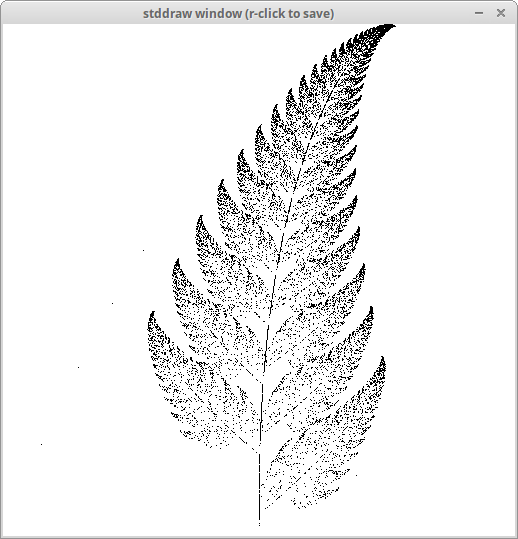
\includegraphics[scale=0.17]{figures/barnsley.png}
\end{center}
\end{minipage}
\end{frame}

\begin{frame}[fragile]
Tree:

\begin{minipage}{160pt}
\begin{lstlisting}[language={}]
$ more tree.txt
6
   0.1  0.1  0.2  0.2  0.2  0.2 
6 3
   0.00  0.00  0.550
  -0.05  0.00  0.525
   0.46 -0.15  0.270
   0.47 -0.15  0.265
   0.43  0.28  0.285
   0.42  0.26  0.290
6 3
   0.00  0.60  0.000
  -0.50  0.00  0.750
   0.39  0.38  0.105
   0.17  0.42  0.465
  -0.25  0.45  0.625
  -0.35  0.31  0.525
$ python ifs.py 20000 < tree.txt
\end{lstlisting}
\end{minipage}%
\begin{minipage}{140pt}
\hfill 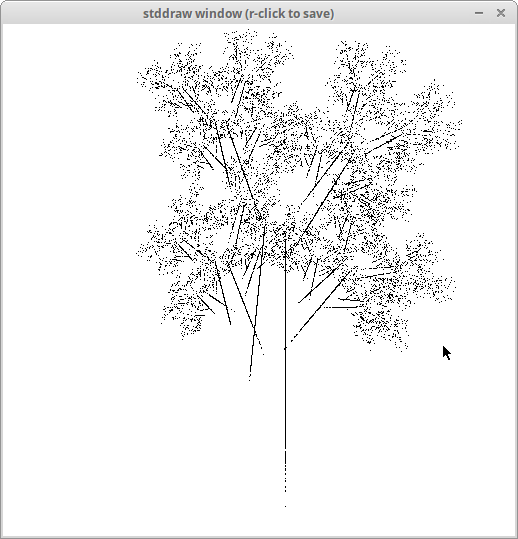
\includegraphics[scale=0.17]{figures/tree.png}
\end{minipage}

\bigskip

Coral:

\begin{minipage}{160pt}
\begin{lstlisting}[language={}]
$ more coral.txt
3
   0.40  0.15  0.45 
3 3
   0.307692 -0.531469  0.8863493
   0.307692 -0.076923  0.2166292
   0.000000  0.545455  0.0106363
3 3
  -0.461538 -0.293706  1.0962865
   0.153846 -0.447552  0.3383760
   0.692308 -0.195804  0.3808254
$ python ifs.py 20000 < coral.txt
\end{lstlisting}
\end{minipage}%
\begin{minipage}{140pt}
\hfill 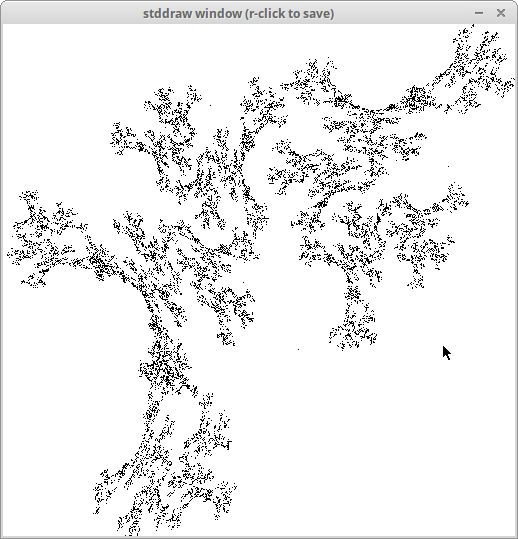
\includegraphics[scale=0.17]{figures/coral.png}
\end{minipage}
\end{frame}

\begin{frame}[fragile]
\begin{framed}
\tiny bernoulli.py: Accept integers $n$ and $trials$ as command-line arguments. Perform $trials$ experiments, each of which counts the number of heads found when a fair coin is flipped $n$ times. Then draw the results to standard draw. 
\end{framed}

\begin{lstlisting}[language=Python]
import gaussian
import math
import stdarray
import stddraw
import stdrandom
import stdstats
import sys

def main():
    n = int(sys.argv[1])
    trials = int(sys.argv[2])
    freq = stdarray.create1D(n + 1, 0)
    for t in range(trials):
        heads = stdrandom.binomial(n, 0.5)
        freq[heads] += 1
    norm = stdarray.create1D(n + 1, 0.0)
    for i in range(n + 1):
        norm[i] = 1.0 * freq[i] / trials
    phi = stdarray.create1D(n + 1, 0.0)
    stddev = math.sqrt(n) / 2.0
    for i in range(n + 1):
        phi[i] = gaussian.pdf(i, n / 2.0, stddev)
    stddraw.setCanvasSize(1000, 400)
    stddraw.setYscale(0, 1.1 * max(max(norm), max(phi)))
    stdstats.plotBars(norm)
    stdstats.plotLines(phi)
    stddraw.show()

if __name__ == '__main__':
    main()
\end{lstlisting}
\end{frame}

\begin{frame}[fragile]
\begin{minipage}{160pt}
\begin{lstlisting}[language={}]
$ python bernoulli.py 20 100000
\end{lstlisting}
\end{minipage}%
\begin{minipage}{140pt}
\hfill 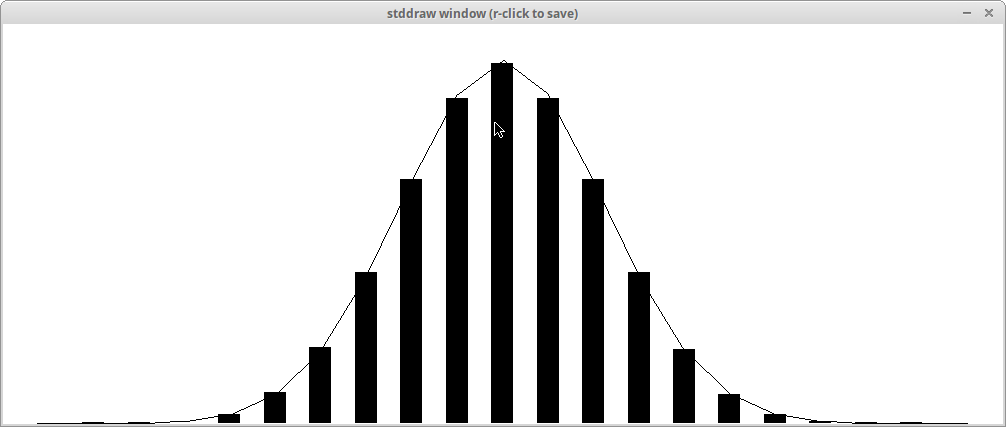
\includegraphics[scale=0.12]{figures/bernoulli.png}
\end{minipage}
\end{frame}


\end{document}
